\documentclass[compress, mathserif, fleqn, 10pt]{beamer}
\useoutertheme{split}
\useoutertheme[subsection=false]{smoothbars}
\useinnertheme[shadow=true]{rounded}
\usecolortheme{whale}
\usecolortheme{orchid}

\setbeamerfont{block title}{size={}}
\setbeamertemplate{navigation symbols}{}
\beamersetuncovermixins{\opaqueness<1->{15}}{}
% \setbeamertemplate{page number in head/foot}[totalframenumber]

\makeatletter
\let\beamer@writeslidentry@miniframeson=\beamer@writeslidentry%
\def\beamer@writeslidentry@miniframesoff{%
	\expandafter\beamer@ifempty\expandafter{\beamer@framestartpage}{}% does not happen normally
	{%else
		
		
		% removed \addtocontents commands
		\clearpage\beamer@notesactions%
} }
\newcommand*{\miniframeson}{\let\beamer@writeslidentry=\beamer@writeslidentry@miniframeson}
\newcommand*{\miniframesoff}{\let\beamer@writeslidentry=\beamer@writeslidentry@miniframesoff}
\makeatother

\setlength{\mathindent}{0.5cm}
\setcounter{tocdepth}{2}

\usepackage[utf8]{inputenc}
\usepackage{amsmath}
\usepackage{color}
\usepackage{hhline}
\usepackage{epstopdf}
\usepackage{animate}
\usepackage{textpos}
\usepackage{enumerate}
\usepackage{tikz}

\title{Transformers and Multi-features Time2Vec for Financial Prediction}
\author[Bui Nguyen Kim Hai, Nguyen Duy Chien]{Bui Nguyen Kim Hai, Nguyen Duy Chien}
%\institute{Department of Numerical Analysis, Faculty of Informatics\\ ELTE Eötvös Loránd University, Budapest, Hungary}
\date{\scriptsize \emph{TDK CONFERENCE – IT SCIENCE SECTION, 2024 SPRING}\\
	\bigskip
	Budapest, Hungary\\ May 29, 2024}

\begin{document}
	\abovedisplayskip=1pt \belowdisplayskip=2pt \abovedisplayshortskip=1pt \belowdisplayshortskip=2pt
	
	\begin{frame}
		\titlepage
	\end{frame}
	
	\begin{frame}
		\frametitle{Outline}
		\tableofcontents
	\end{frame}
	
	\section{Introduction}
	\begin{frame}
		\frametitle{Outline}
		\tableofcontents[currentsection]
	\end{frame}
	
	\begin{frame}{Motivation: Cross-correlation to NASDAQ}
		\centerline{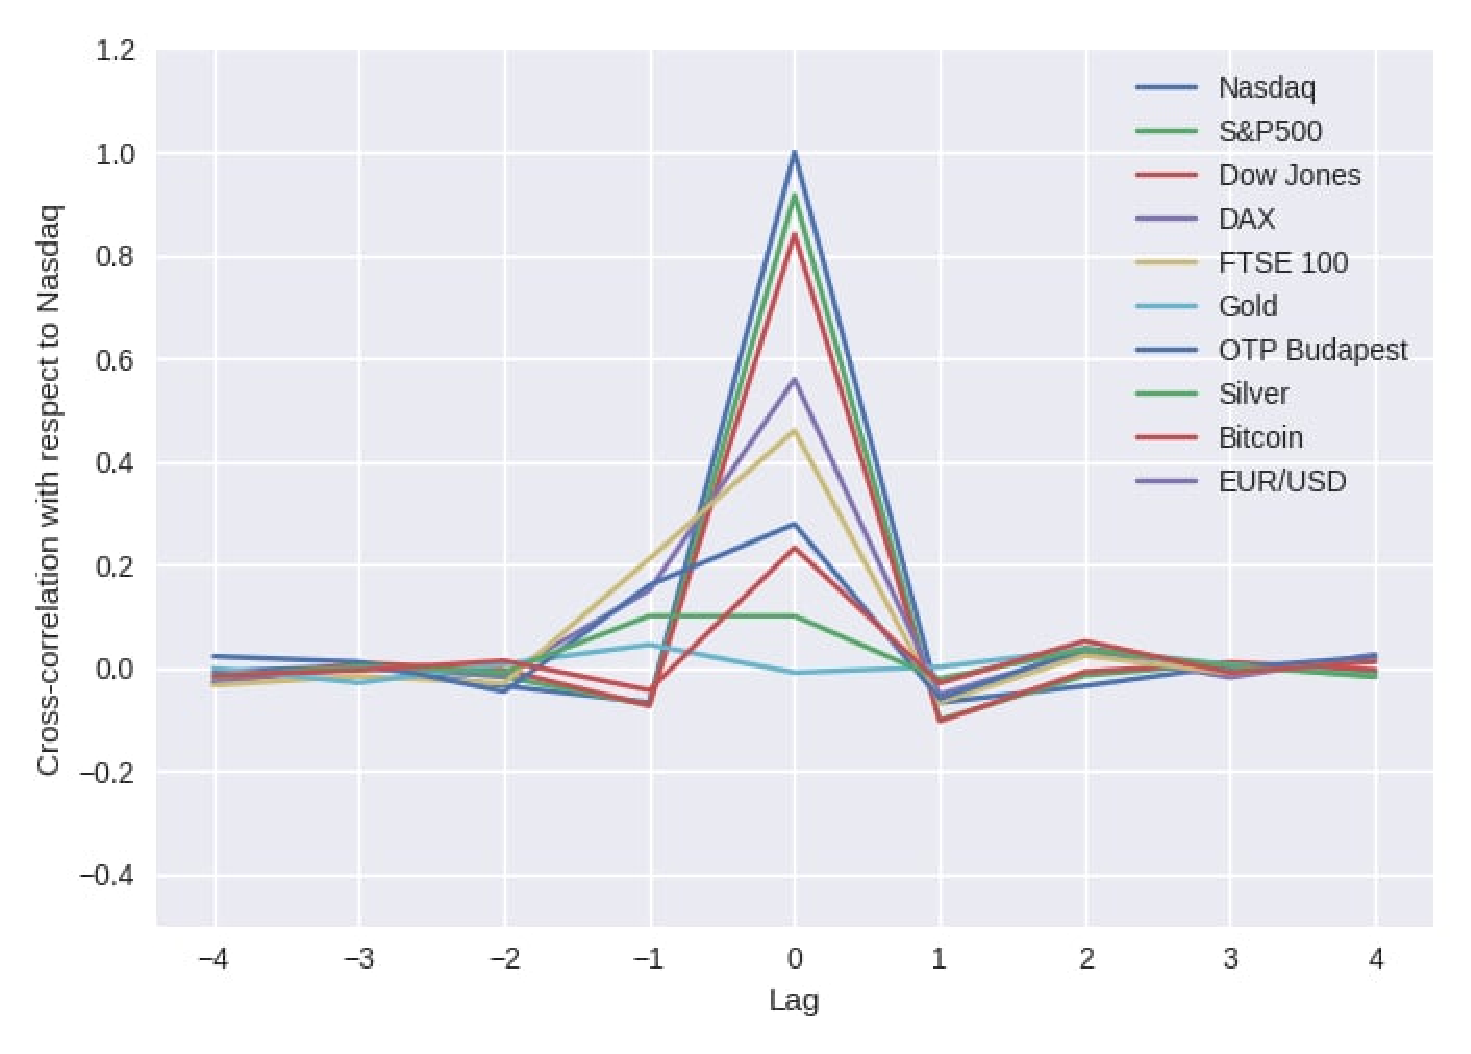
\includegraphics[width=0.85\textwidth]{images/nas_base.eps}}
	\end{frame}
	
	\begin{frame}{Motivation: Cross-correlation to Exxon Mobil}
		\centerline{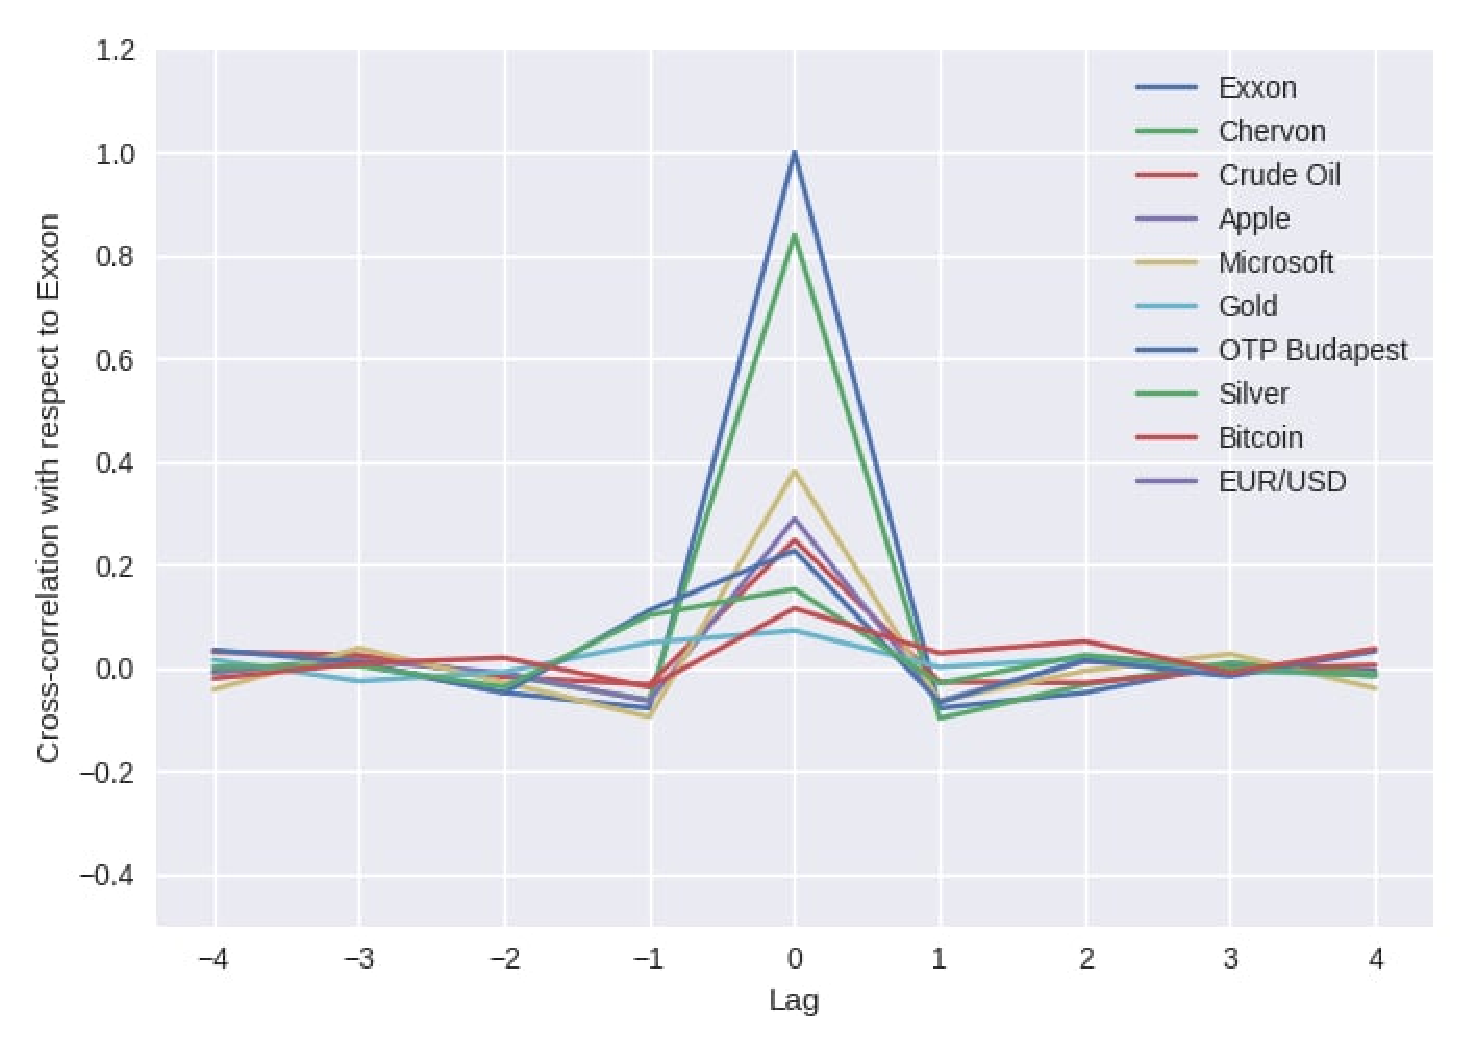
\includegraphics[width=0.85\textwidth]{images/exx_base.eps}}
	\end{frame}
	
	\subsection{Motivation}
	\begin{frame}{Motivation}
		\begin{block}{By other works}
			\begin{itemize}
				\item Researchers try to combine Time2Vec with CNN, RNN, LSTM, and
				Attention mechanism
				
				\item For instances:
				
				\begin{itemize}
					\item Aeroengine Risk Assessment
					
					\item Predicting Production in Shale and Sandstone Gas Reservoirs
					
					\item Stock Price Forecasting
				\end{itemize}
			\end{itemize}
		\end{block}
		\smallskip
		\begin{block}{In finance area}
			\begin{itemize}
				\item Studies primarily rely on one dataset
			\end{itemize}
		\end{block}
		\smallskip
		\begin{block}{By observing trends}
			\begin{itemize}
				\item Stock's trend is a Markov process
				
				\item Historical data offers limited foresight
				
				\item Stocks having similar trend is more promising
			\end{itemize}
		\end{block}
	\end{frame}
	
	\subsection{Related work}
	\begin{frame}{Related work}
		\begin{block}{ARIMA}
			Making one-step-ahead predictions
		\end{block}
		\begin{block}{RNN}
			Handling temporal problems in sequential data and time-series analysis.
		\end{block}
		\begin{block}{LSTM}
			Using gates, LSTM enables network to learn long-term dependencies and
			prevent the vanishing gradient problem.
		\end{block}
		\begin{block}{Transformer}
			The SOTA architecture that works well in many area such as NLP, and time-series
		\end{block}
		\begin{block}{Time2Vec}
			Use to embed the time-series data to vector
		\end{block}
	\end{frame}
	
	\section{Proposed model and techniques}
	\begin{frame}
		\frametitle{Outline}
		\tableofcontents[currentsection]
	\end{frame}
	
	%\subsection{Behavioral similarity of stocks}
	%\begin{frame}{Behavioral similarity of stocks}
	
	%\end{frame}
	
	\subsection{Data collection}
	\begin{frame}{Data collection}
		\begin{exampleblock}{Where to collect?}
			Yahoo Finance
		\end{exampleblock}
		\begin{exampleblock}{What will be collected?}
			Date, Open, High, Low, Close, Volume columns
		\end{exampleblock}
		\begin{exampleblock}{How many datasets should we collect?}
			Two, three, four ..., as long as they are highly correlated to each other
		\end{exampleblock}
		\begin{block}{Collected datasets}
			\begin{itemize}
				\item \structure{Group1}: NASDAQ, S\&P500, DJI, DAX
				
				\item \structure{Group2}: Exxon Mobil, Chervon
			\end{itemize}
		\end{block}
	\end{frame}
	
	\subsection{Preprocessing data}
	\begin{frame}{Preprocessing data: The pipeline}
		\centerline{\includegraphics[width=0.8\paperwidth]{images/pipeline-big.eps}}
		\centerline{The preprocessing data pipeline.}
		\begin{block}{Techniques}
			\begin{itemize}
				\item \structure{Fill-forward}: Filling missing data in dataset
				
				\item \structure{Moving Average}: Smoothing dataset by averaging data
				
				\item \structure{Percentage Change}: Compute the difference in the data
				
				\item \structure{Min-Max Normalization}: Normalizing dataset
				
				\item \structure{Geometry Mean Not NaN (GMNN)}: Combining multiple datasets
			\end{itemize}
		\end{block}
	\end{frame}
	
	\subsection{Model architecture}
	\begin{frame}{Model architecture: Proposed model}
		\begin{columns}
			\begin{column}{0.45\textwidth}
				\centerline{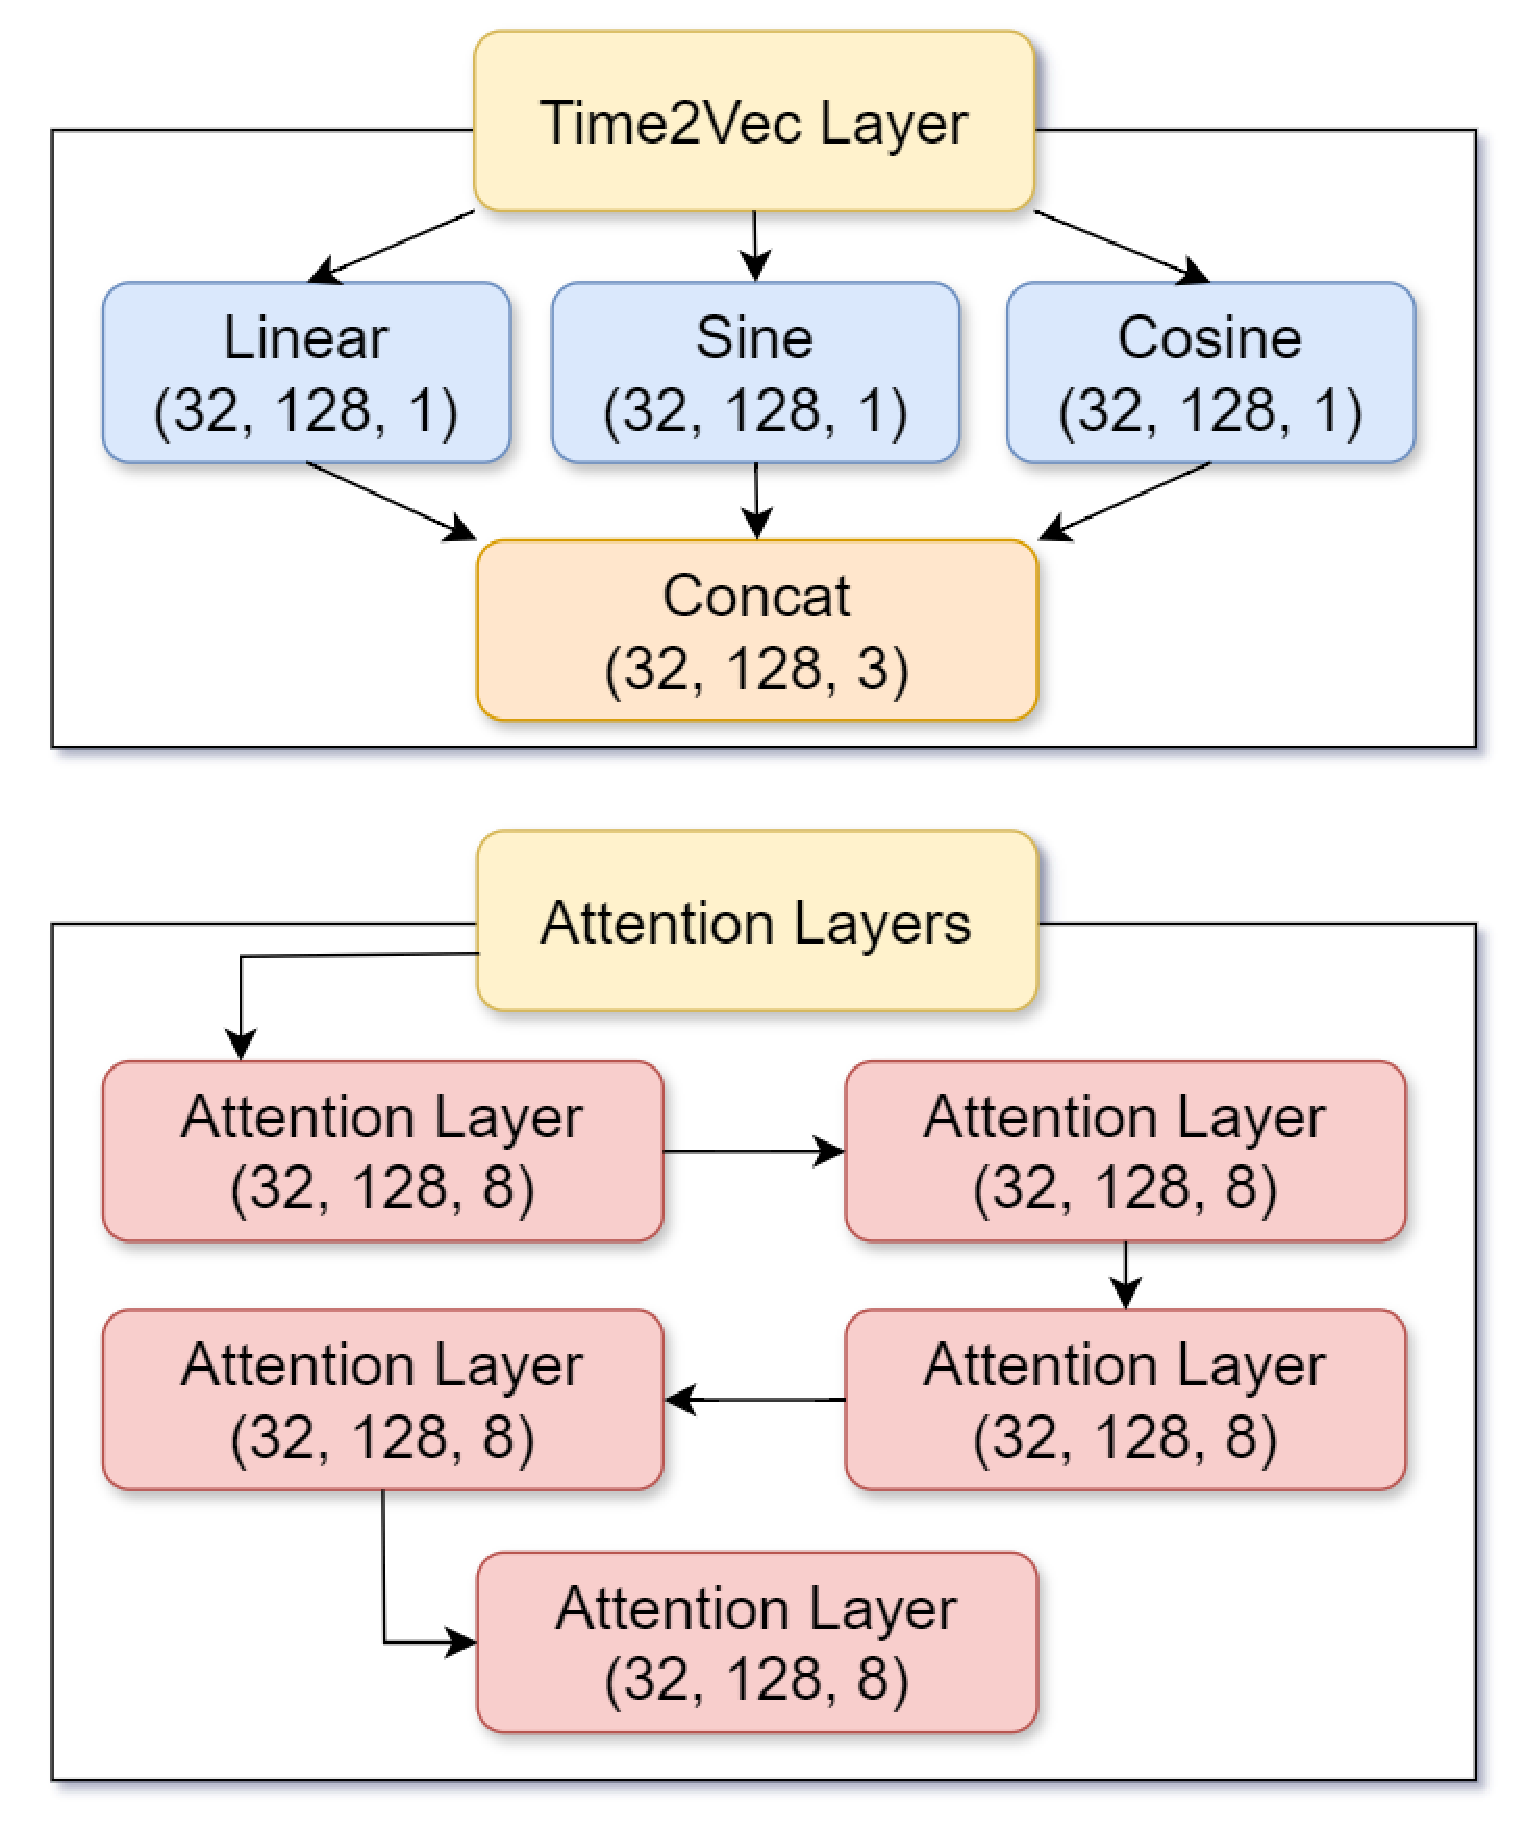
\includegraphics[width=\textwidth]{images/model-parts.eps}}
			\end{column}
			\begin{column}{0.45\textwidth}
				\centerline{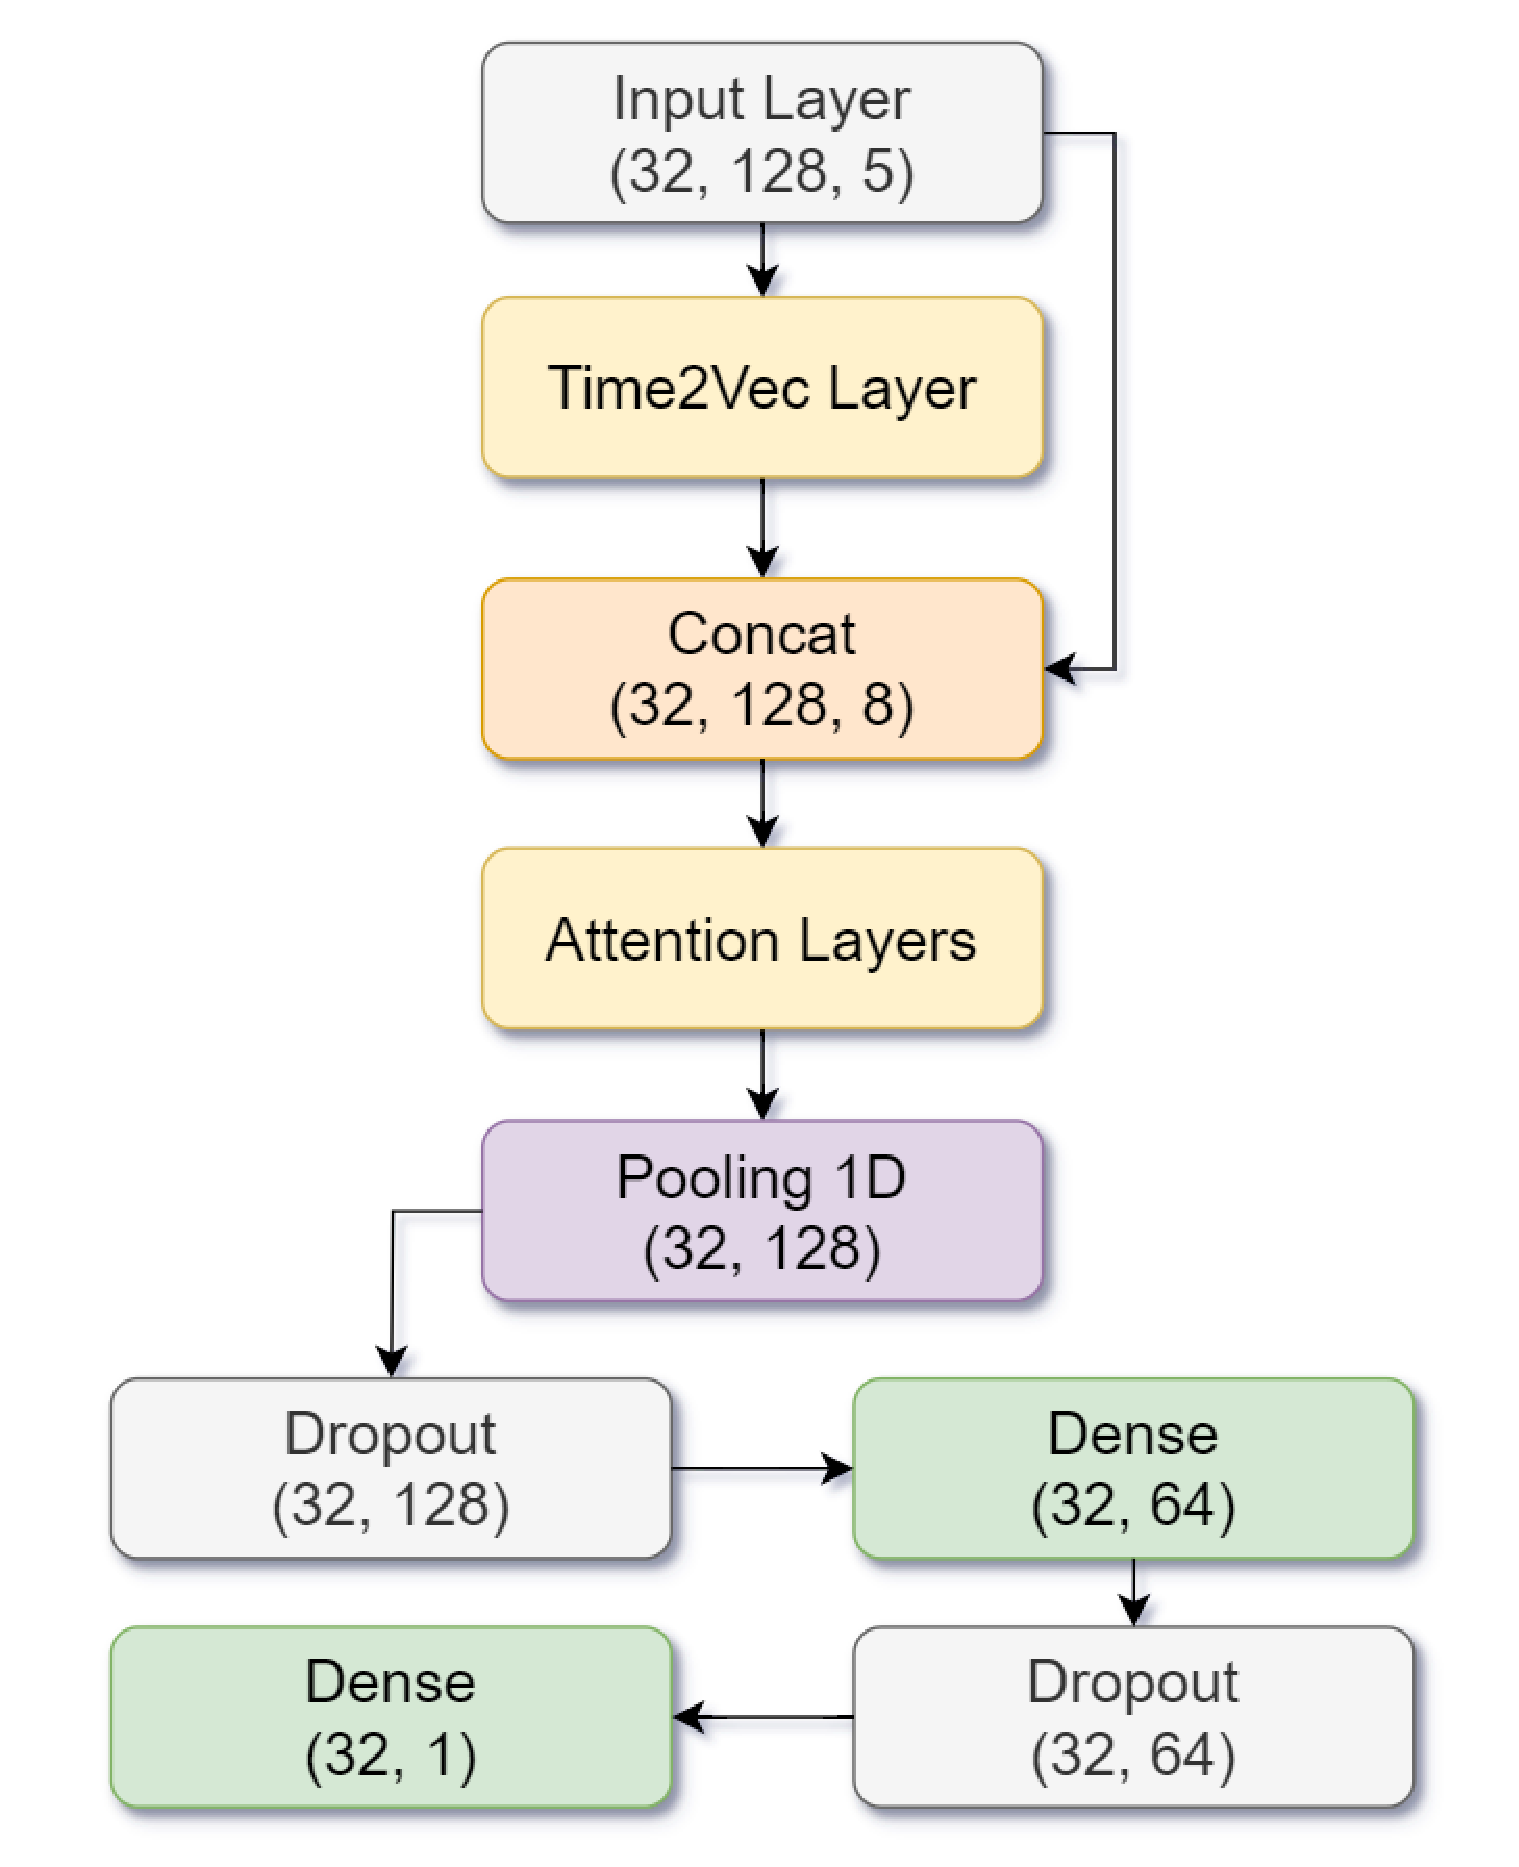
\includegraphics[width=\textwidth]{images/model-mini.eps}}
			\end{column}
		\end{columns}
	\end{frame}
	
	\begin{frame}{Model architecture: Role of layers}
		\begin{columns}
			\begin{column}{0.45\textwidth}
				\centerline{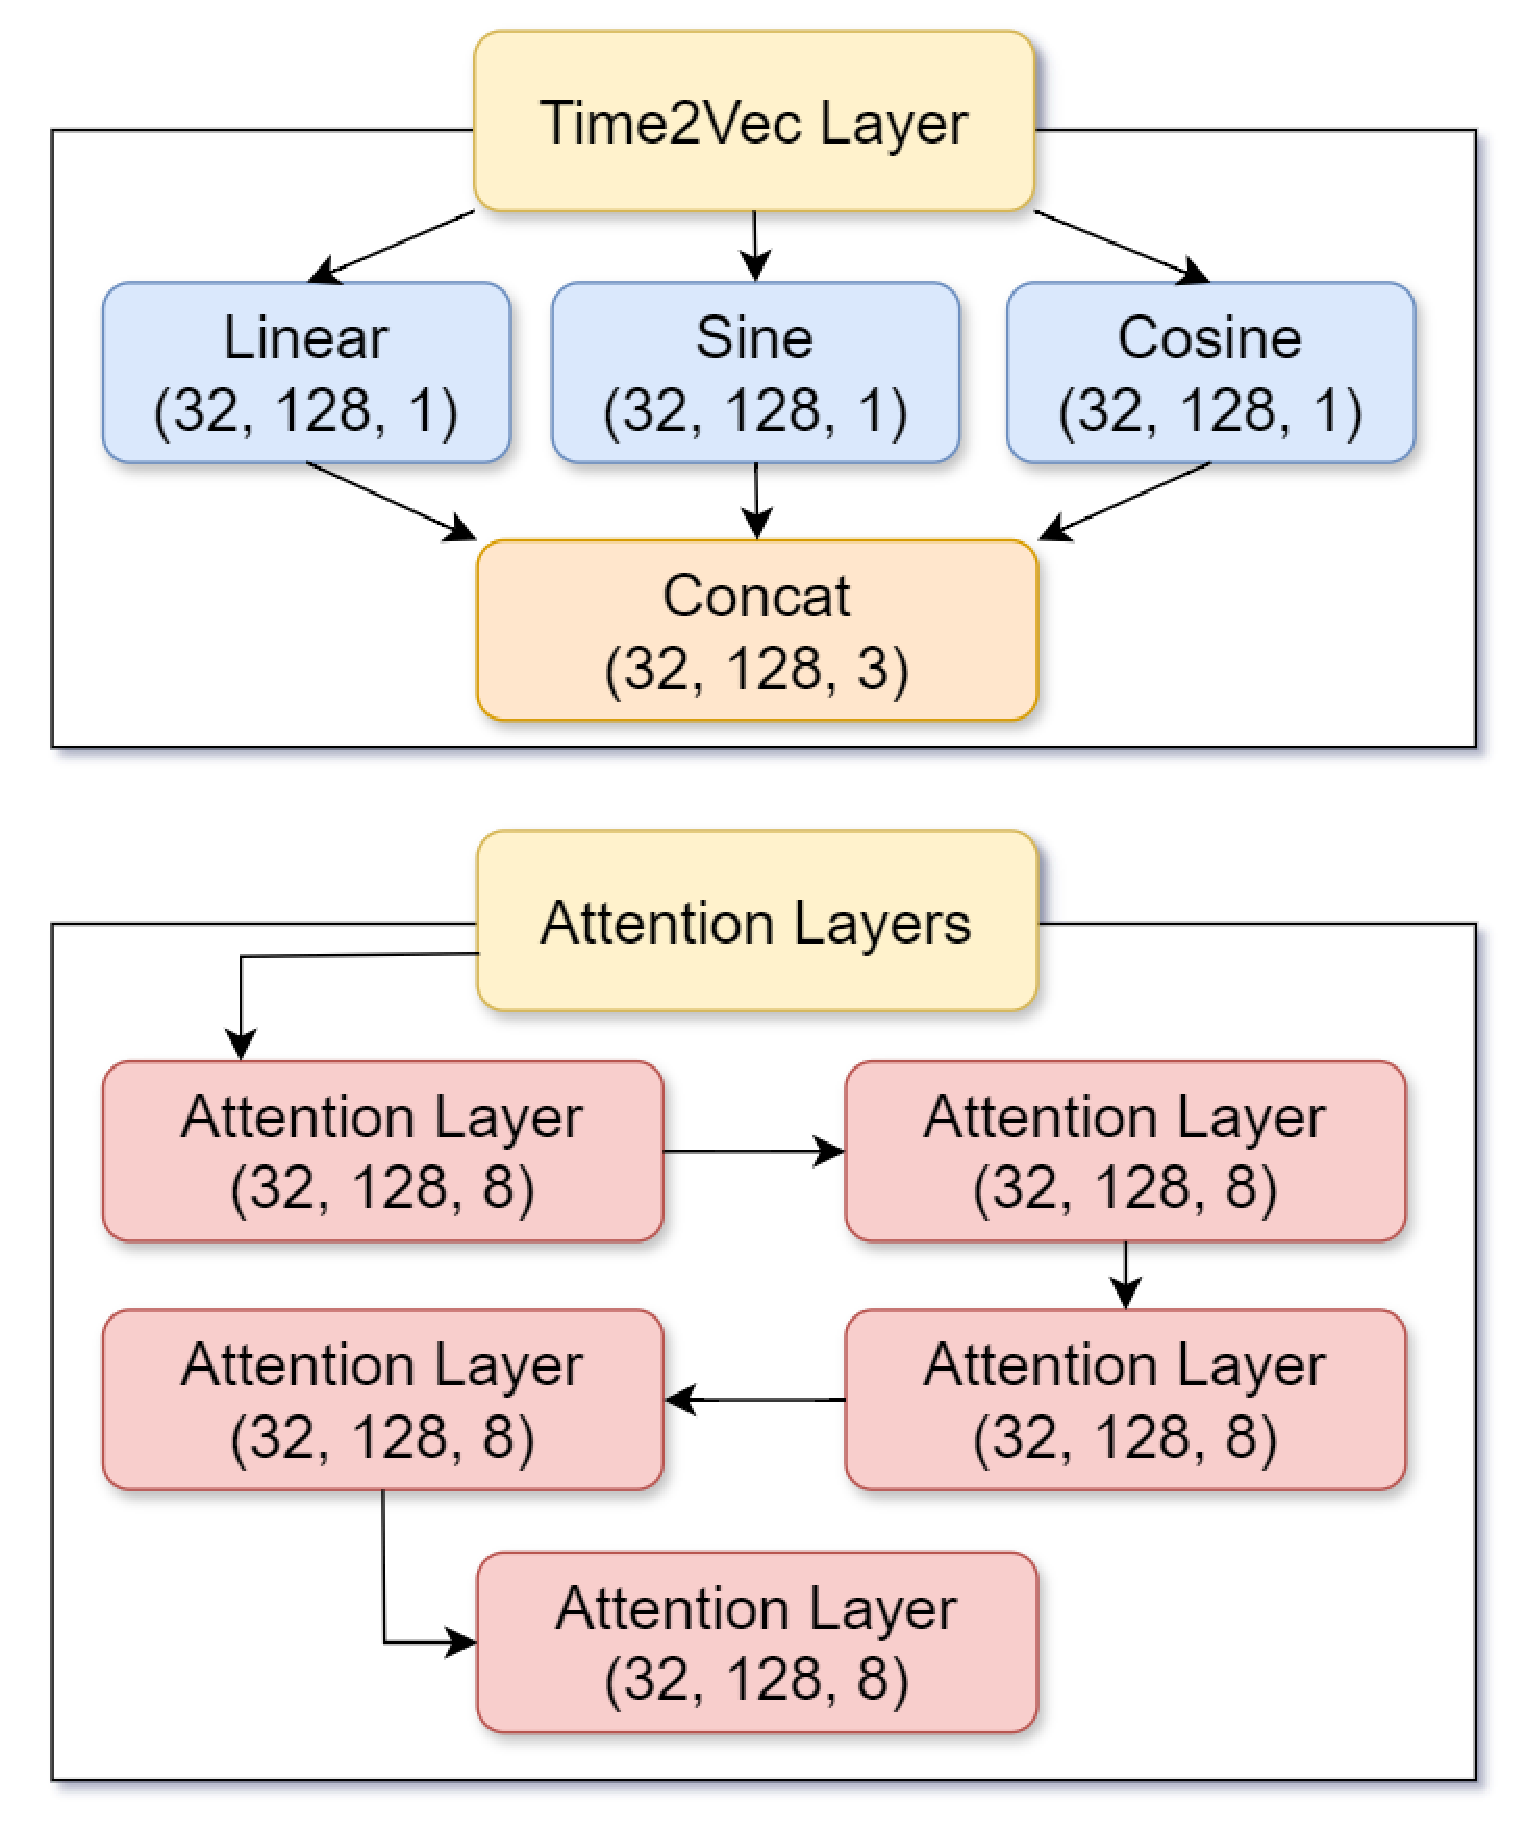
\includegraphics[width=\textwidth]{images/model-parts.eps}}
			\end{column}
			\begin{column}{0.55\textwidth}
				\begin{block}{Roles}
					\begin{itemize}
						\item \structure{Time2Vec}
						\begin{itemize}
							\item \structure{Linear}: Capturing linear trends
							\smallskip
							
							\item \structure{Sine, Cosine}: Encoding positions and capturing
							periodic behaviors
							\smallskip
							
							\item \structure{Concat}: Concatenating above three layers
						\end{itemize}
						\bigskip
						
						\item \structure{Attention Layers}
						\begin{itemize}
							\item To study the trend from different aspects, positions
							\smallskip
						\end{itemize}
					\end{itemize}
				\end{block}
			\end{column}
		\end{columns}
	\end{frame}
	
	\begin{frame}{Model architecture: Role of layers}
		\begin{columns}
			\begin{column}{0.55\textwidth}
				\begin{block}{Roles}
					\begin{itemize}
						\item \structure{Time2Vec}: Catch continuous attribute of time
						
						\item \structure{Concat}: Apply Residual Connection
						
						\item \structure{Attention}: Deep understanding trend movements
						
						\item \structure{Pooling}: Reducing dimension
						
						\item \structure{Dropout}: Prevent over-fitting
						
						\item \structure{Dense}: Apply activation functions (ReLU)
					\end{itemize}
				\end{block}
			\end{column}
			\begin{column}{0.45\textwidth}
				\centerline{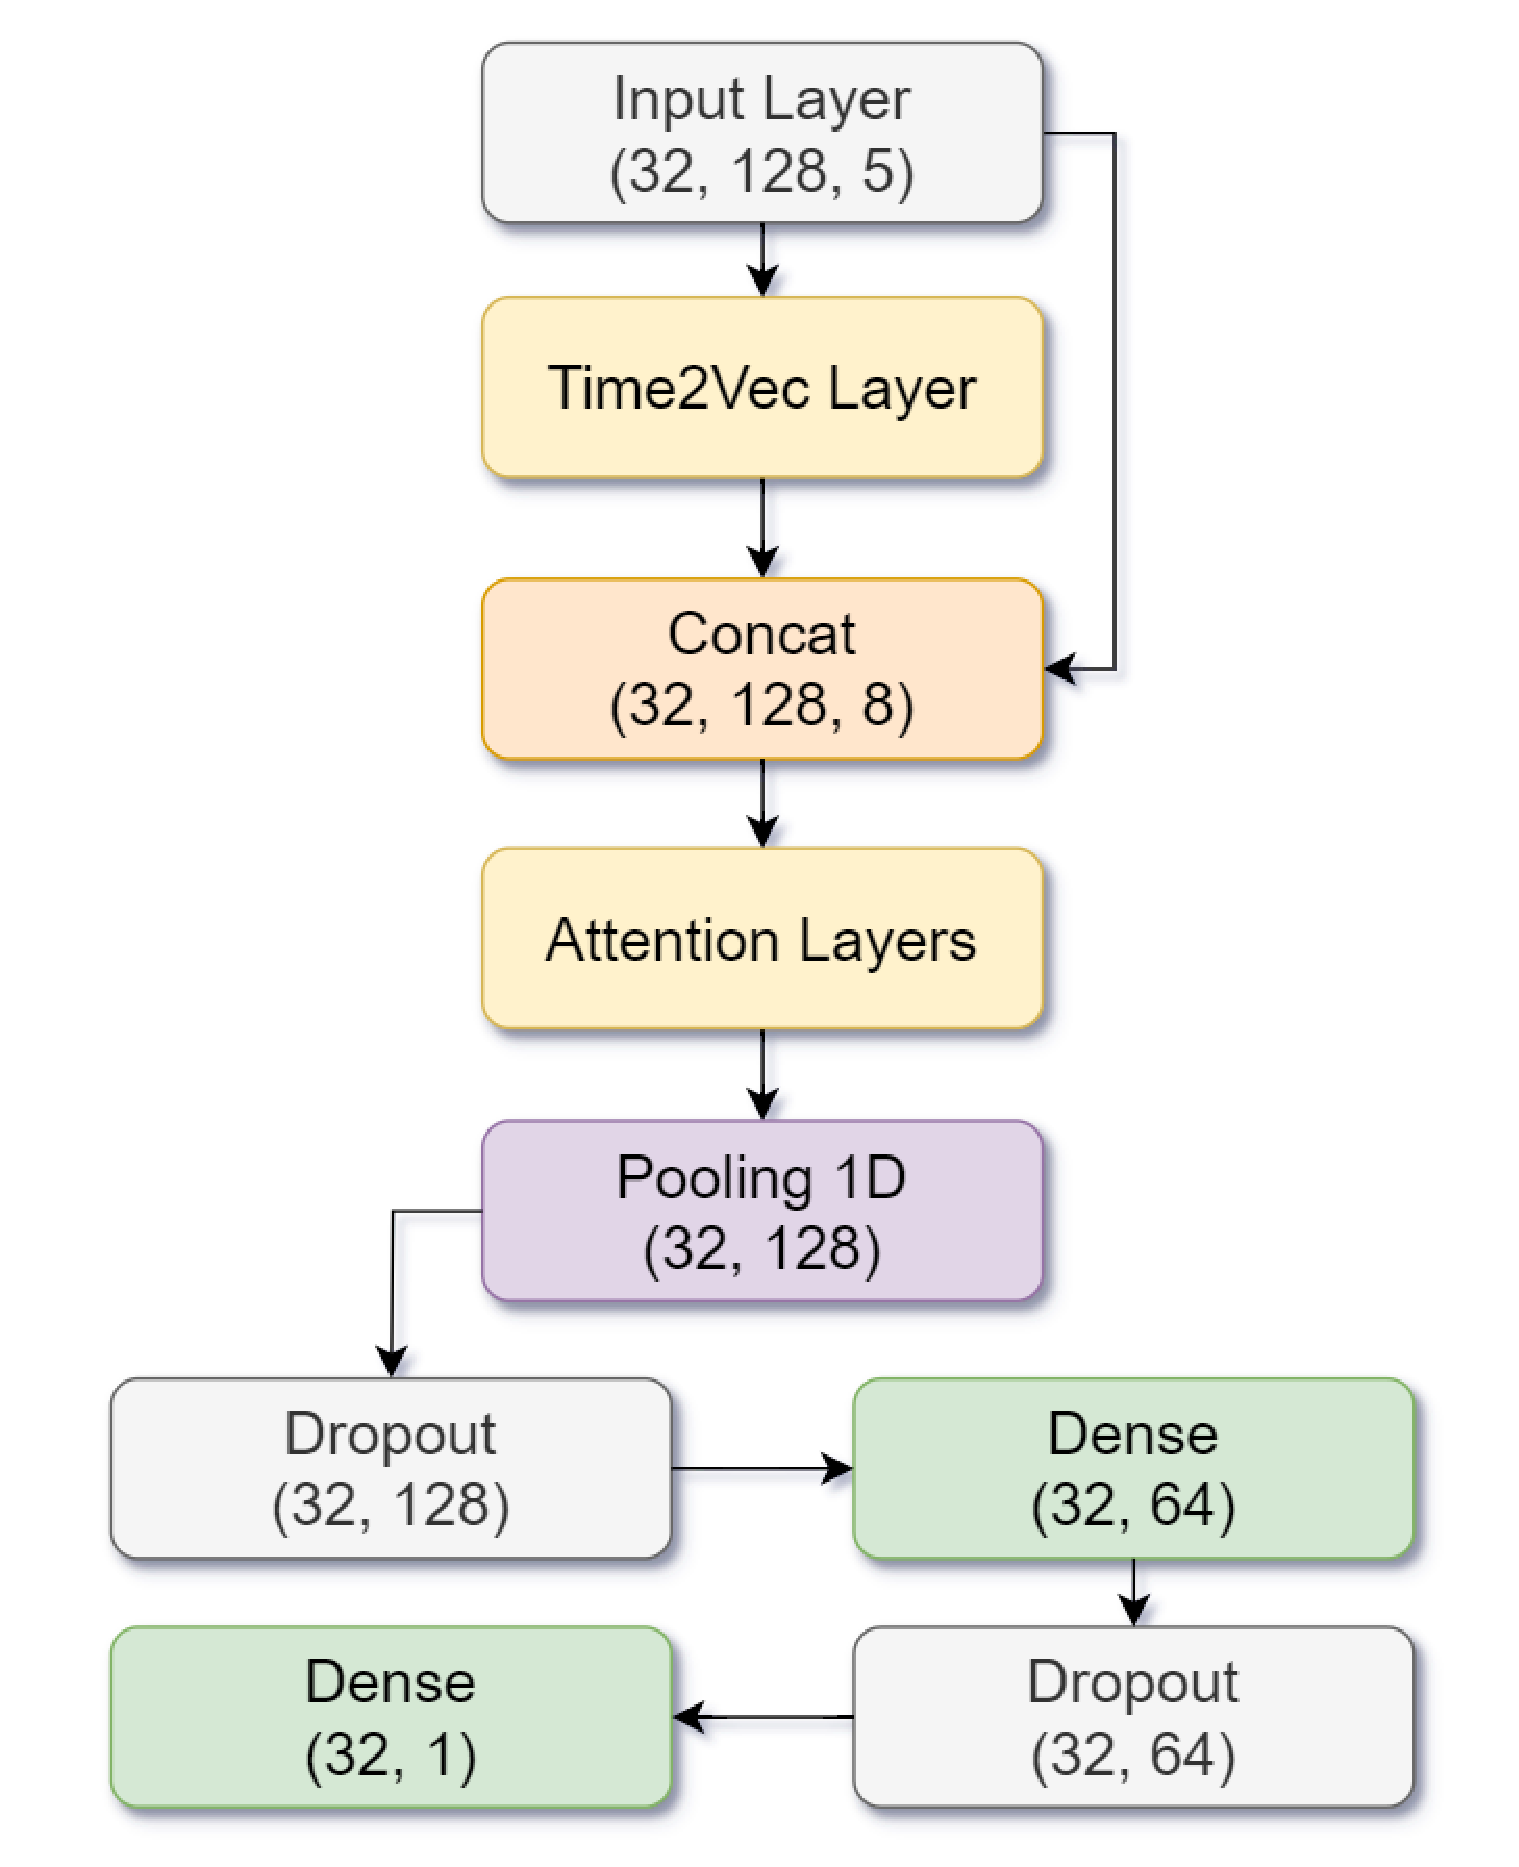
\includegraphics[width=\textwidth]{images/model-mini.eps}}
			\end{column}
		\end{columns}
	\end{frame}
	
	\subsection{Decoding engineering}
	\begin{frame}{Decoding engineering}
		\centerline{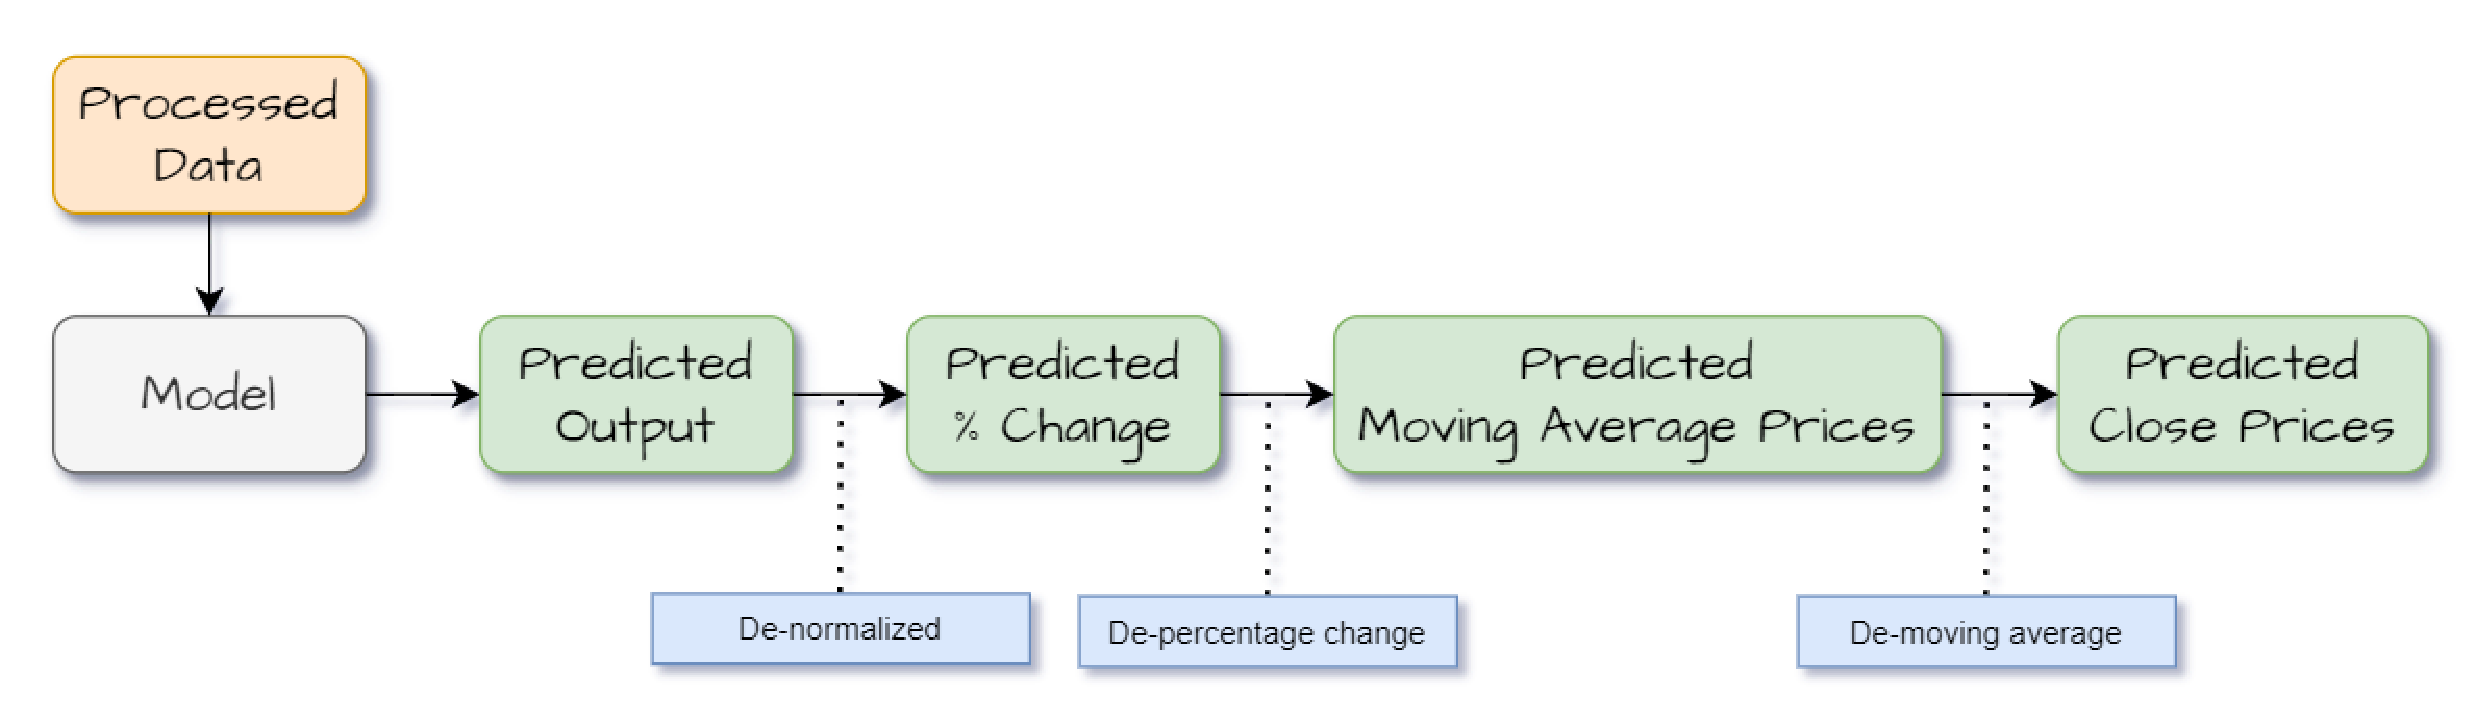
\includegraphics[width=0.8\paperwidth]{images/decode.eps}}
		\centerline{The decoding pipeline.}
		\begin{columns}
			\begin{column}{0.5\textwidth}
				\begin{block}{Techniques}
					\begin{minipage}[t][2cm][t]{\textwidth}
						\begin{itemize}
							\item De-normalized
							
							\item De-percentage change
							
							\item De-moving average
						\end{itemize}
					\end{minipage}
				\end{block}
			\end{column}
			\begin{column}{0.5\textwidth}
				\begin{exampleblock}{Why don't we use De-GMNN step?}
					\begin{minipage}[t][2cm][t]{\textwidth}
						\begin{itemize}
							\item Output is \textbf{normalized} (Invariant)
							
							\item Target is \textbf{one} dataset, output only reflects that one
						\end{itemize}
					\end{minipage}
				\end{exampleblock}
			\end{column}
		\end{columns}
	\end{frame}
	
	\section{Results and Conclusion}
	\begin{frame}{Outline}
		\tableofcontents[currentsection]
	\end{frame}
	
	\begin{frame}
		\frametitle{Conclusion}
		\begin{block}{Conclusion}
			\smallskip
			By leveraging multiple criteria to evaluate the proposed model such as
			\begin{itemize}
				\item MAE, MAPE, RMSE, MSE, R2-score (price prediction task)
				\smallskip
				
				\item Accuracy (trend forecasting task)
			\end{itemize}
			\bigskip
			
			We can proudly say that, the multi-feature model
			\begin{itemize}
				\item \textbf{Outperforms} the single-feature one in most cases and they
				are \textbf{extremely close} to each other in other scenarios.
				\smallskip
				
				\item Usually yields \textbf{better} result than the SOTA in almost
				every contexts.
			\end{itemize}
			\smallskip
		\end{block}
	\end{frame}
	
	\begin{frame}{Results}
		\begin{columns}
			\begin{column}{0.5\textwidth}
				\centerline{\includegraphics[width=1.12\textwidth]{images/exxon-big.eps}}
			\end{column}
			\begin{column}{0.5\textwidth}
				\centerline{\includegraphics[width=1.12\textwidth]{images/nasdaq-big.eps}}
			\end{column}
		\end{columns}
		
		\smallskip
		\centerline{Comparing 6 metrics with respect to Exxon (Left), NASDAQ (Right)}
	\end{frame}
	
	\section{Summary}
	\begin{frame}
		\frametitle{Outline}
		\tableofcontents[currentsection]
	\end{frame}
	
	\begin{frame}{Summary}
		\begin{exampleblock}{Summary}
			\begin{itemize}
				\item We explore deep learning for challenging stock price prediction
				
				\item Paving the way for new feature studies and applications in various
				deep learning models
				
				\item Demonstrates correlation-based features and innovative neural networks
				improve stock price prediction
			\end{itemize}
		\end{exampleblock}
		
		\begin{block}{Further Research}
			\begin{itemize}
				\item Fine-tuning the architecture
				
				\item Continuing improving processing methods
				
				\item Comparing to other SOTA neural networks like KAN
				
				\item Applying the architecture to other areas
			\end{itemize}
		\end{block}
	\end{frame}
	\miniframesoff
	\section*{}
	\begin{frame}
		\begin{beamercolorbox}
			[sep=8pt,center,shadow=true,rounded=true]{title} \usebeamerfont{title}Thank
			you for your attention!\par%
		\end{beamercolorbox}
	\end{frame}
	
	\begin{frame}{But... What is GMNN?}
		\begin{columns}
			\begin{column}{0.5\textwidth}
				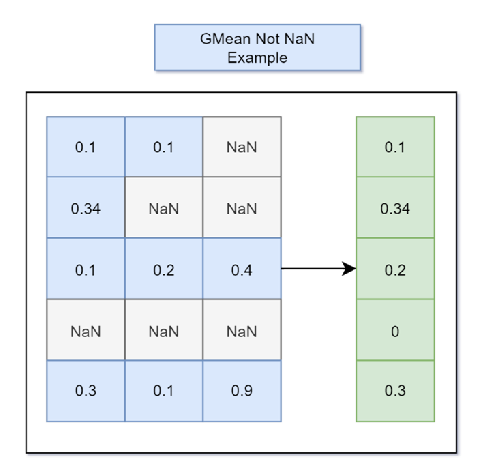
\includegraphics[width=\textwidth]{images/gmnn.eps}
			\end{column}
			\begin{column}{0.5\textwidth}
				\begin{block}{GMNN Attributes}
					\begin{itemize}
						\item \structure{Union}: Handling length difference when combining datasets
						\smallskip
						
						\item \structure{Invariant}: Keeping the data stays normalized
						\smallskip
						
						\item \structure{Representation}: The output reflects the whole datasets
						\smallskip
					\end{itemize}
				\end{block}
				\vspace*{1cm}
			\end{column}
		\end{columns}
		\bigskip
		\centerline{A simple sample of applying GMNN transformation}
	\end{frame}
	
	\begin{frame}{But... What is Time2Vec\footnote[1]{Seyed Mehran Kazemi et al. “Time2Vec:
				Learning a Vector Representation of Time” (2019)}?}
		\begin{block}{Time2Vec}
			An approach providing a model – agnostic vector representation for time
		\end{block}
		
		\begin{block}{Time2Vec Function}
			\centering
			{ $\textbf{t2v}(\tau)[i]=\left\{\begin{array}{cc}w_i \tau+\varphi_i & \text{ if } i=0 \\ F \left(w_i \tau+\varphi_i\right), & \text{ if } 1 \leq i \leq k\end{array}\right.$ }
			
			\smallskip
			
			$w, \varphi$: learnable parameters \space $\tau$: time
			
			$F$: periodic activation function (eg. $\sin, \cos$)
		\end{block}
		
		\begin{block}{Time2Vec Attributes}
			\begin{itemize}
				\item Capturing both periodic and non periodic patterns
				
				\item Being invariant to time re-scaling
				
				\item Being simple enough so it can be combined with many models
			\end{itemize}
		\end{block}
	\end{frame}
	
	\begin{frame}{Splitting data}
		\begin{exampleblock}{Can we just put the processed data into model straight
				forward?}
			No, we can not feed the whole data straight forward into the model, because
			that action will cause \textbf{over-fitting} problem which no one want it
			to be happened when training model
		\end{exampleblock}
		
		\begin{block}{Do we need to shuffle the data before splitting?}
			No, we don't want to shuffle the data because it has \textbf{continuous} attribute
			of time then shuffling will make the data lose this special and important property
			which cause a big problem for the model to learn the pattern
		\end{block}
		
		\begin{exampleblock}{How will we feed input data to our model?}
			We will split the data into three categories:
			\begin{itemize}
				\item \structure{Train}: The first 80\% data of the input
				
				\item \structure{Validation}: The next 10\% data
				
				\item \structure{Test}: The last 10\% data
			\end{itemize}
		\end{exampleblock}
	\end{frame}
	
	\begin{frame}{Applications}
		\begin{block}{Can it be used in production?}
			Of course, but to be more accurate and precise, the architecture must be fine-tuned
			to fit the expectation
		\end{block}
		
		\begin{exampleblock}{Is it easy to set up and use in production?}
			Yes it is, developer just need to find the appropriate datasets and train
			the model
		\end{exampleblock}
		
		\begin{block}{Can it be used in other areas?}
			Yes it can be used in other areas, we just need to find the dimension
			sizes and appropriate hyper-parameters to fit the area expectation
		\end{block}
		
		\begin{exampleblock}{Can it predict the tomorrow stock price?}
			Yes it can, but we need to apply some more techniques to decode back to
			real values
		\end{exampleblock}
	\end{frame}
	
	\begin{frame}{Questions}
		\begin{block}{From the reviewer}
			\begin{itemize}
				\item \structure{Correlation method}: We use the default one in pandas (Pearson)
				
				\item \structure{Source of Equations and formulas in Decoding part}: They
				are just applying the reverse logic of how we coding it. That's why we
				don't use any citation for these in our thesis
			\end{itemize}
		\end{block}
	\end{frame}
	
	\begin{frame}{Explain correlation method}
		\begin{block}{Pearson}
			Considering two time series $y(t)$ and $x(t)$ with an equal length of $T$ ($1
			< t < T$), the Pearson's correlation coefficient between the series is
			defined as
			
			\bigskip
			
			\centerline{$\rho=\frac{\sum_{t=1}^{t=T}(x(t)-\bar{x})(y(t)-\bar{y})}{\sqrt{\sum_{t=1}^{t=T}(x(t)-\bar{x})^{2}} \sqrt{\sum_{t=1}^{t=T}(y(t)-\bar{y})^{2}}}$}
			\bigskip
			where $\bar{x}$ and $\bar{y}$ are average values over the whole series
			
			\smallskip
			
			A higher value of Pearson’s correlation coefficient $\rho$ positively corresponds
			with the stronger correlation degree, thereby indicating a stronger mutual
			interpretation ability between $y(t)$ and $x(t)$
		\end{block}
		
		\begin{exampleblock}{}
			However, when time series are nonstationary and nonlinear, the Pearson's correlation
			coefficient cannot represent a reliable correlation degree because the observational
			values in the time series probably rely on each other.
		\end{exampleblock}
	\end{frame}
	
	\begin{frame}{Explain used techniques: De-normalized}
		\begin{block}{De-normalized step}
			\centerline{$x_{pct}=x_{nor}\times(max-min)+min \label{de-nor}$}
			\bigskip
			
			\centerline{Is from}
			
			\bigskip
			\centerline{$x_{standarlized}=\frac{x-\min (x)}{\max (x)-\min (x)}$}
			
			\smallskip
			Where:
			
			\begin{itemize}
				\item $x_{pct}$ has the same role with $x$
				
				\item $x_{nor}$ has the same role with $x_{standardlized}$
				
				\item $max$ is stored value of $\max(x)$
				
				\item $min$ is stored value of $\min(x)$
			\end{itemize}
		\end{block}
		
		\begin{exampleblock}{But... why?}
			Because
			\begin{itemize}
				\item Before standardlizing, our $x$ is currently percentage-changed
			\end{itemize}
		\end{exampleblock}
	\end{frame}
	
	\begin{frame}{Explain used techniques: De-percentage change - Problem}
		\begin{block}{De-percentage change step}
			This is the way we \textbf{create} to get high accuracy predict values by
			pairing with real values to decode
			
			Why? Let's see how we encode percentage change
		\end{block}
		\smallskip
		\centerline{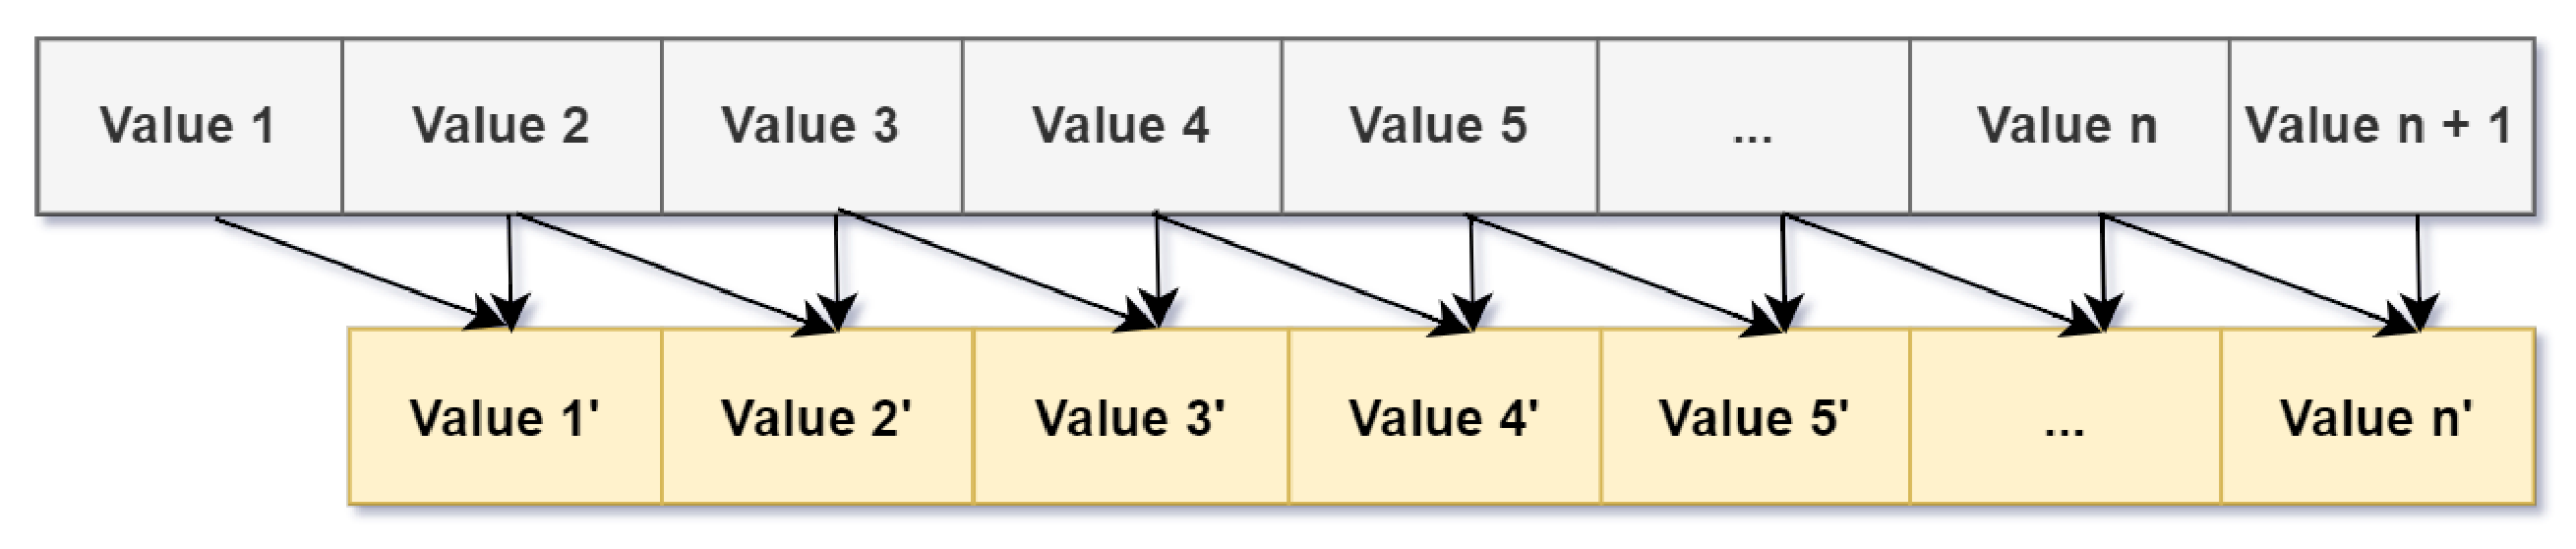
\includegraphics[width=\textwidth]{images/enc_percent.eps}}
		\bigskip
		\begin{exampleblock}{This lead to a problem!}
			We lost one data cell
		\end{exampleblock}
	\end{frame}
	
	\begin{frame}{Explain used techniques: De-percentage change - Plan A}
		\begin{block}{Plan A to fix}
			This plan will cause a very big mistake when converting back to real prices
			because it one predict is not good, the next ones will be affected too!
		\end{block}
		\smallskip
		\centerline{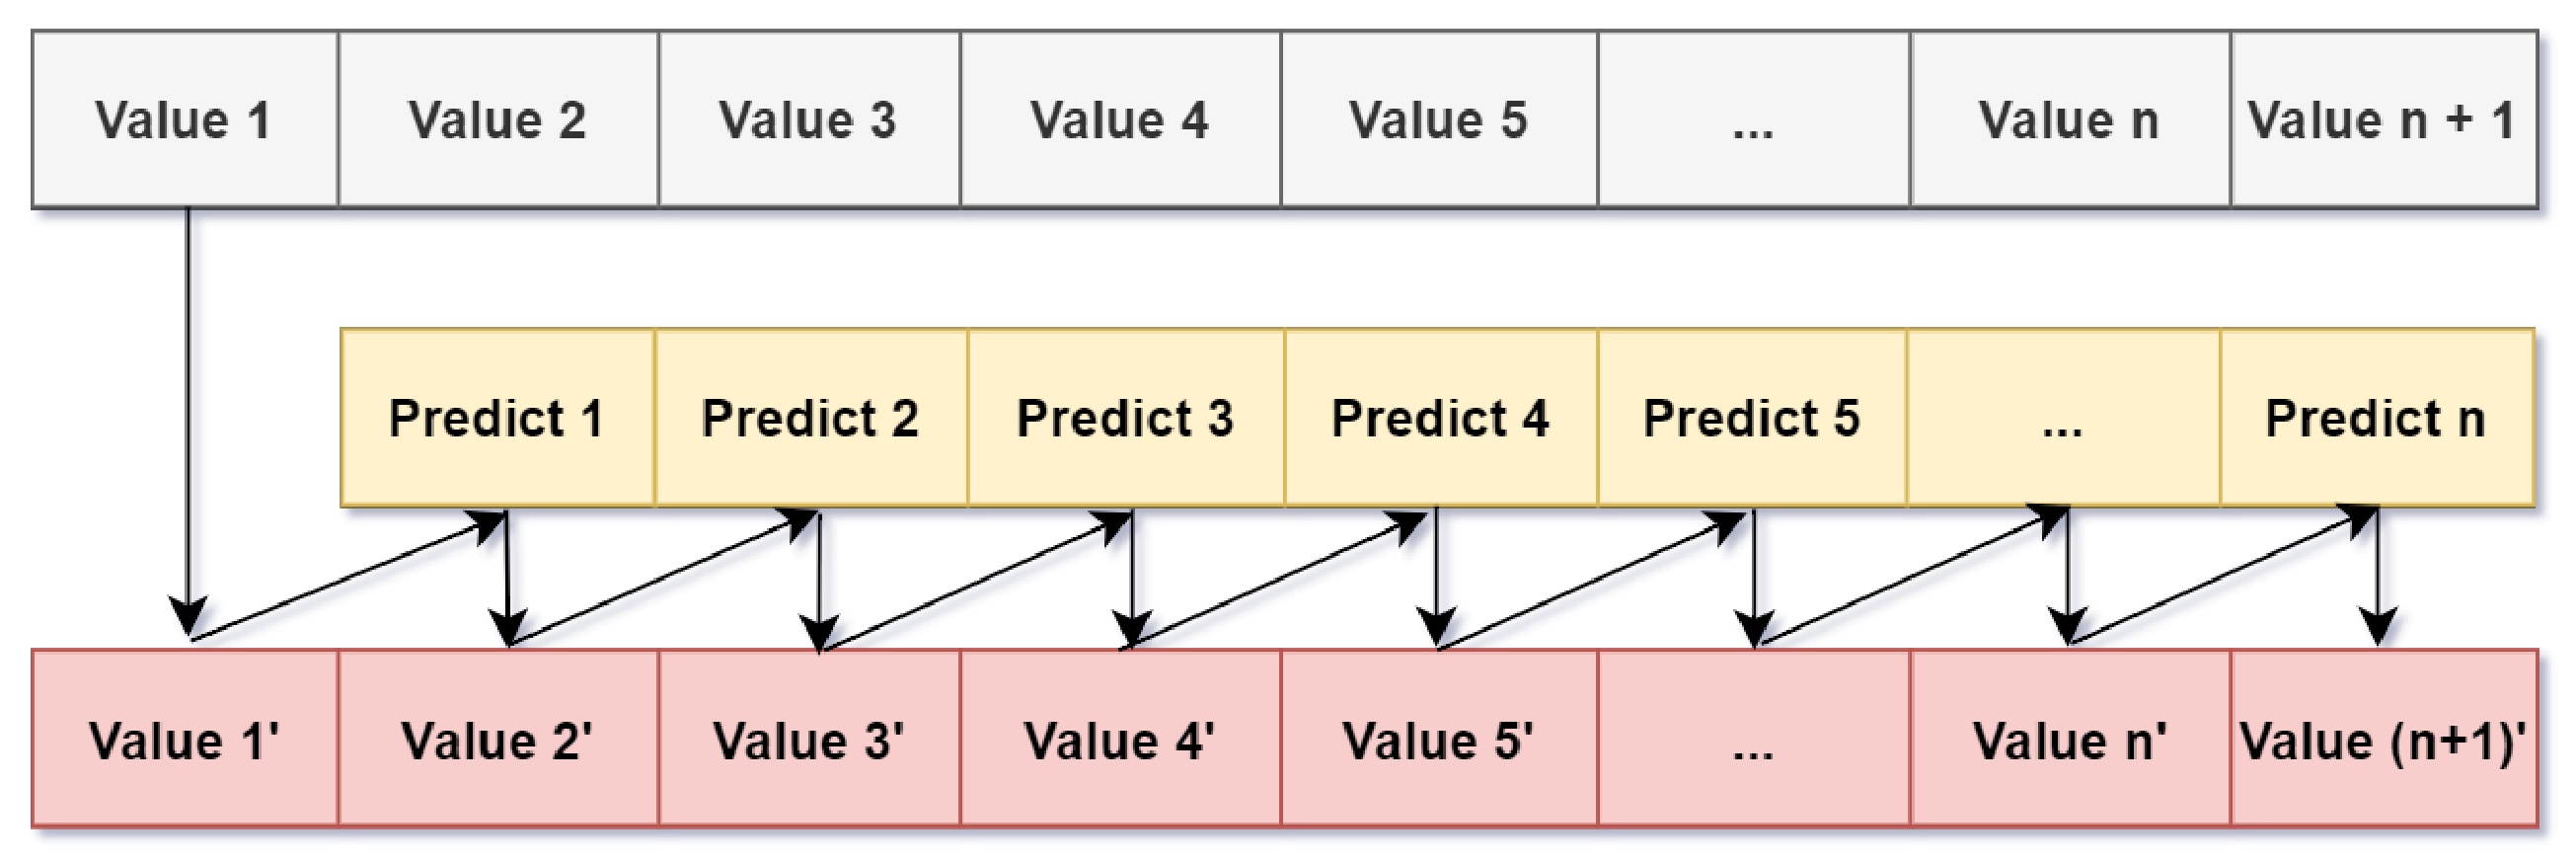
\includegraphics[width=\textwidth]{images/dec_percent_bad.eps}}
		\bigskip
		\begin{exampleblock}{Any plan else?}
			Yes, we will see plan B - which will be better, and that is also the one we
			proposed in the thesis
		\end{exampleblock}
	\end{frame}
	
	\begin{frame}{Explain used techniques: De-percentage change - Plan B}
		\begin{block}{Plan B to fix}
			This plan yields very good result in converting back to real values,
			because each cell is only related to the real one and/or the predict one -
			which is more realistic than plan A
		\end{block}
		\smallskip
		\centerline{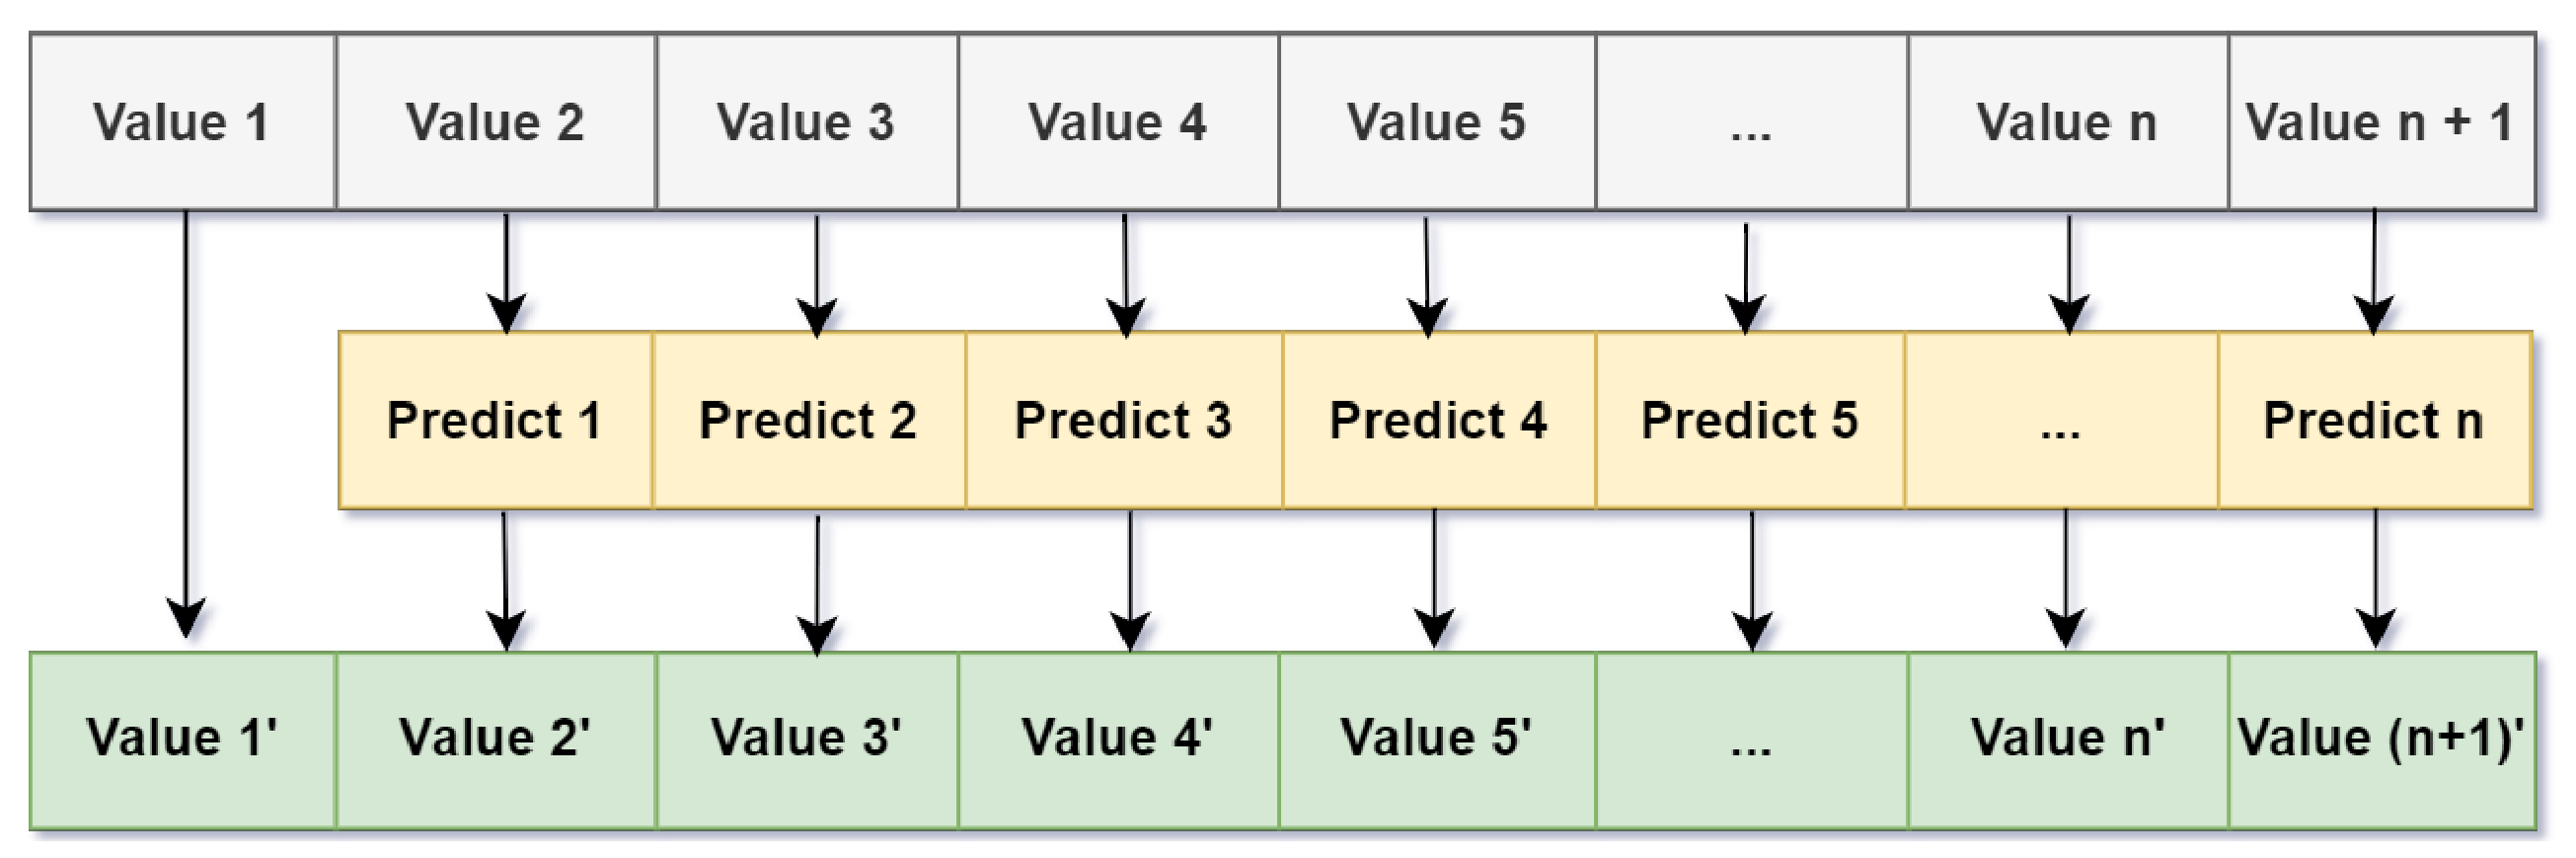
\includegraphics[width=\textwidth]{images/dec_percent_good.eps}}
	\end{frame}
	
	\begin{frame}{Explain used techniques: De-percentage change - Formula}
		\begin{block}{Formula for plan B}
			\centerline{$x_{mva}=\left\{ \begin{array}{l}v_{mva}, i=0 \\ v_{mva} \times\left(1+x_{pct}\right), otherwise\end{array}\right.$}
			
			\smallskip
			
			\centerline{Is from}
			
			\smallskip
			
			\centerline{$x_{pct}=\frac{x_{b} - x_{a}}{x_{a}}$}
			
			\smallskip
			Where:
			
			\begin{itemize}
				\item $x_{a}$, $x_{b}$: is two consecutive moving average values ($x_{b}$
				after $x_{a}$)
				
				\item $x_{pct}$ has the same meaning in two equation
				
				\item $x_{mva}$ has the same role with $x_{a}$, $x_{b}$
				
				($x_{mva}$ is a vector; $x_{a}$, $x_{b}$ are numbers)
				
				\item $v_{mva}$ is real moving average values (from encoding part)
			\end{itemize}
		\end{block}
		
		\begin{exampleblock}{Disclaimer}
			We have a typo in our thesis in this step. We messed up between $v_{vma}$
			with $v_{pct}$
		\end{exampleblock}
	\end{frame}
	
	\begin{frame}{Explain used techniques: De-moving average - Problem}
		\begin{block}{De-moving average step}
			This is the way we \textbf{came up with} to get high accuracy predict
			values by pairing with real values to decode
			
			Why? Let's see how we apply moving average with step equals 14 days
		\end{block}
		\smallskip
		\centerline{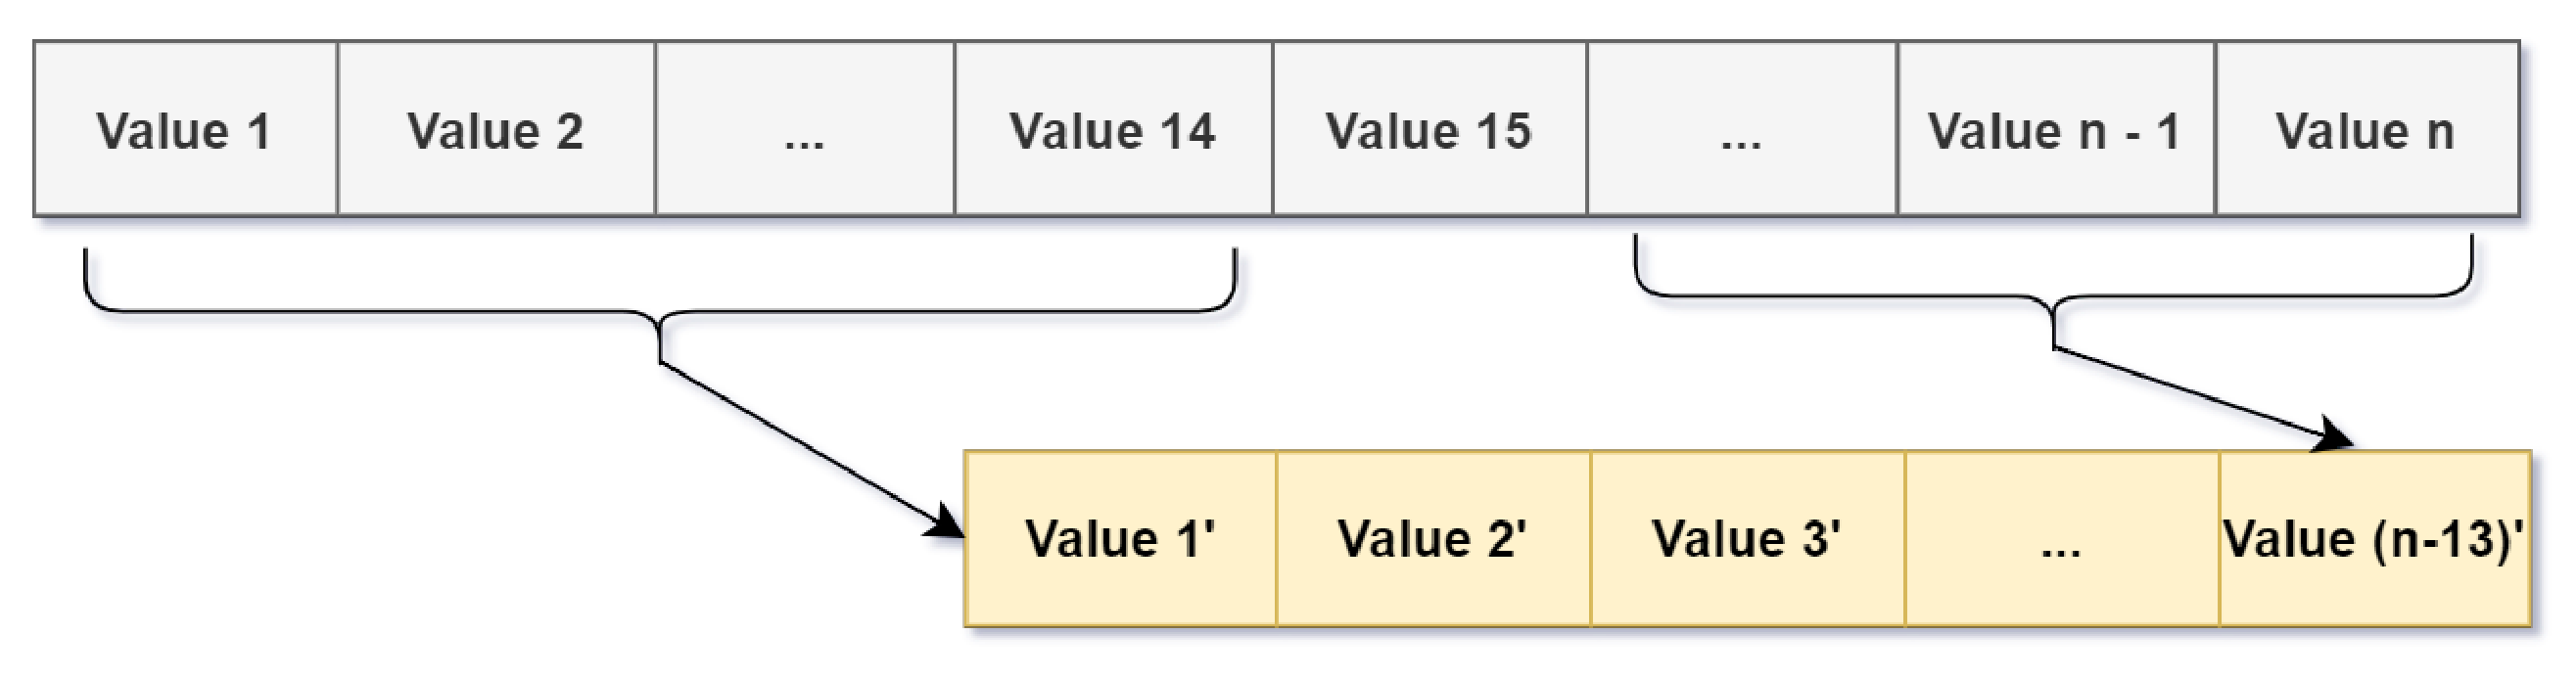
\includegraphics[width=\textwidth]{images/enc_moving.eps}}
		\bigskip
		\begin{exampleblock}{This lead to a problem!}
			We lost the first 13 data cells
		\end{exampleblock}
	\end{frame}
	
	\begin{frame}{Explain used techniques: De-moving average - Fix the problem}
		\begin{block}{De-moving average step}
			This method yields very good result in converting back to real values,
			because each cell is only related to the real one and/or the predict one
		\end{block}
		\smallskip
		\centerline{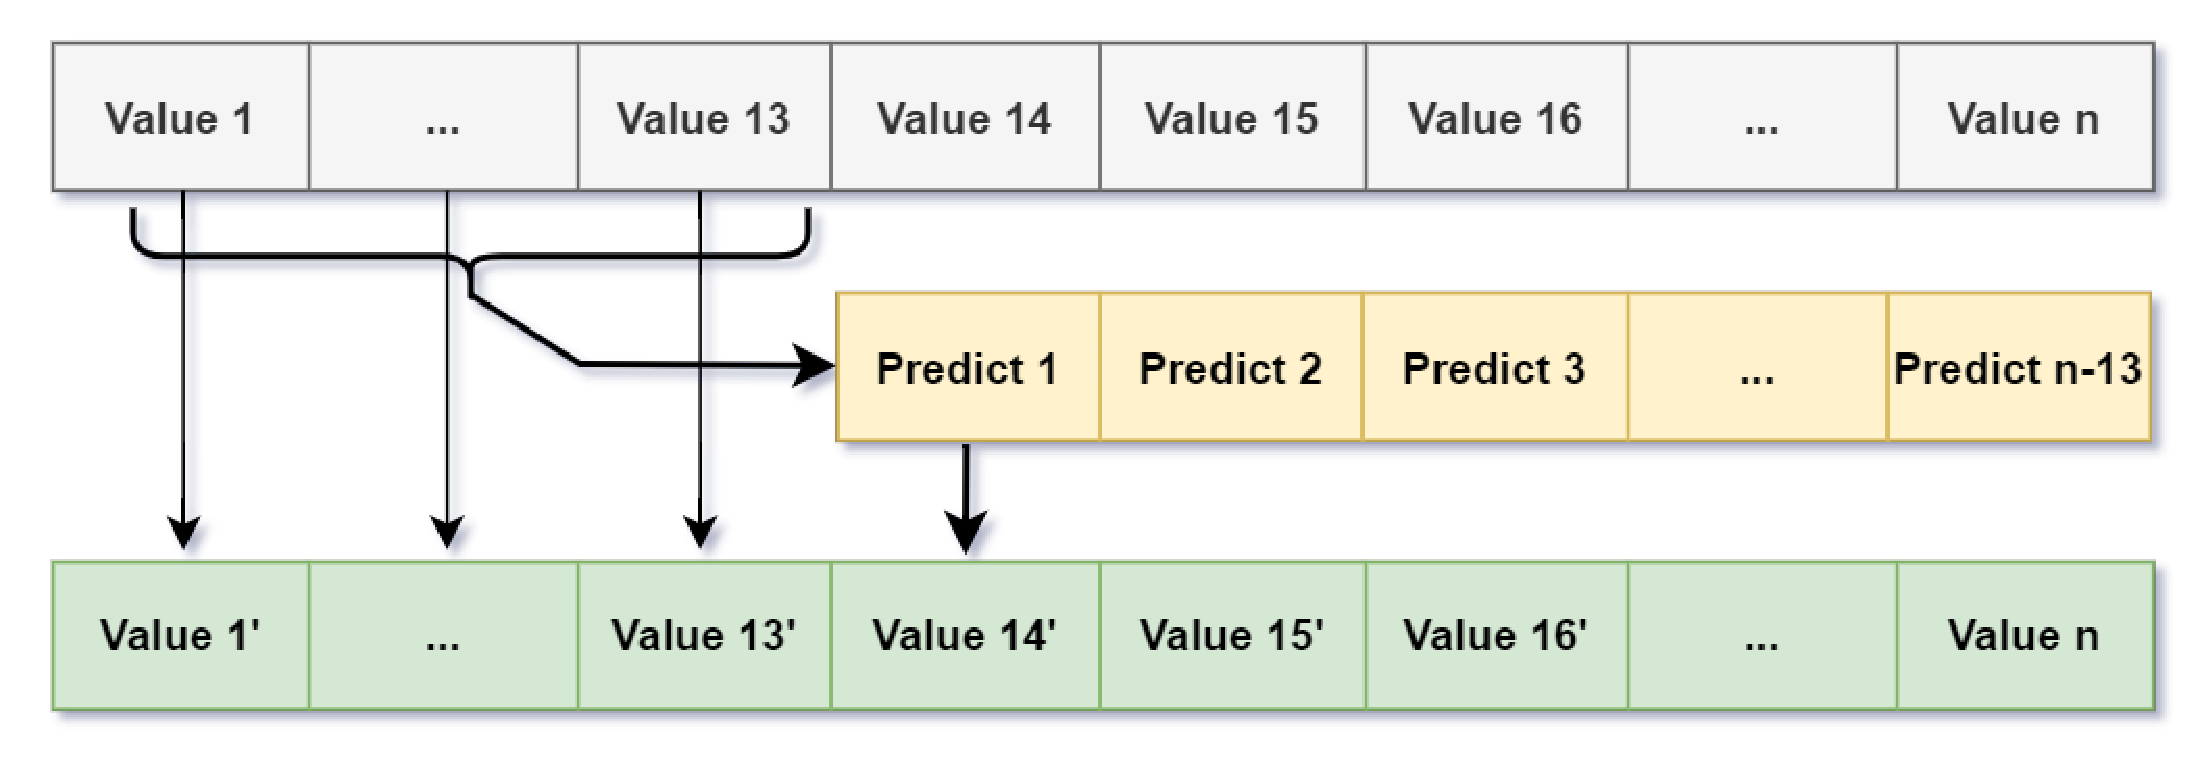
\includegraphics[width=\textwidth]{images/dec_moving.eps}}
		\bigskip
	\end{frame}
	
	\begin{frame}{Explain used techniques: De-moving average - Formula}
		\begin{block}{Formula}
			\centerline{$x_{close}= \begin{cases}v_{close}&, i \leq 13 \\ x_{mva}\times 14&- \sum_{k=i-14}^{i-1}v_{close}, i \geq 14\end{cases}$}
			
			\smallskip
			
			\centerline{Is from}
			
			\smallskip
			
			\centerline{$mva=1/14 * \sum_{0}^{13}close$}
			
			\smallskip
			Where:
			
			\begin{itemize}
				\item $x_{vma}$: has the predict moving average prices
				
				(from the De-percentage change step)
				
				\item $mva$: real moving average prices
				
				\item $v_{close}$, $close$: has the same meaning in two equation, real
				close prices
			\end{itemize}
		\end{block}
	\end{frame}
\end{document}